\section{Collision Avoidance} \label{sec:collision_avoidance}

% \subsection{Disturbance Repulsion}
A crucial property of the proposed controller is its ability to ensure collision avoidance in the presence of external disturbances.



\begin{lemma}
	A dynamical system evolves with the rigid body dynamics given in \eqref{eq:robot_dynamics} controlled by \eqref{eq:control_command}, with damping matrix $\matd{D}$ from \eqref{eq:damping_summation}, and a negligible Coriolis effect.
    A point-like agent starting at position $\vect p = \{{\vecs \xi}\}_0$ close to the surface, i.e., $\Gamma( \vect p) \approx 1$ is guided by a velocity field $\vect f(\vecs \xi)$ parallel to the surface with a starting velocity $\vect v^0= \vect f(\{{\vecs \xi}\}_0)$.
    A large disturbance towards the obstacle results in a velocity of $\{\dot{\vecs \xi}\}_0 = \vect v^I +  \vect v^0$ after the impact, with $\| \vect v^I \| \gg \| \vect v^0 \|$.
	A motion starting in free space remains collision-free for all times, i.e., $\Gamma( \{\vecs \xi_t\}) \geq 1$ with $t \geq 0$ if the impact velocity is limited by $\| \vect v^I\| < s^{\mathrm{o}} \| \vecs \xi - \vecs \xi^b \| / m^{\mathrm{min}}$, with respect to the closes surface point $\vecs \xi^b \in \mathbb{R}^N$ and mass $m \in \mathbb{R}_{>0}$.
\end{lemma}


\begin{figure}[htb]
\centering
 % \begin{subfigure}{0.99\columnwidth}
  \centerline{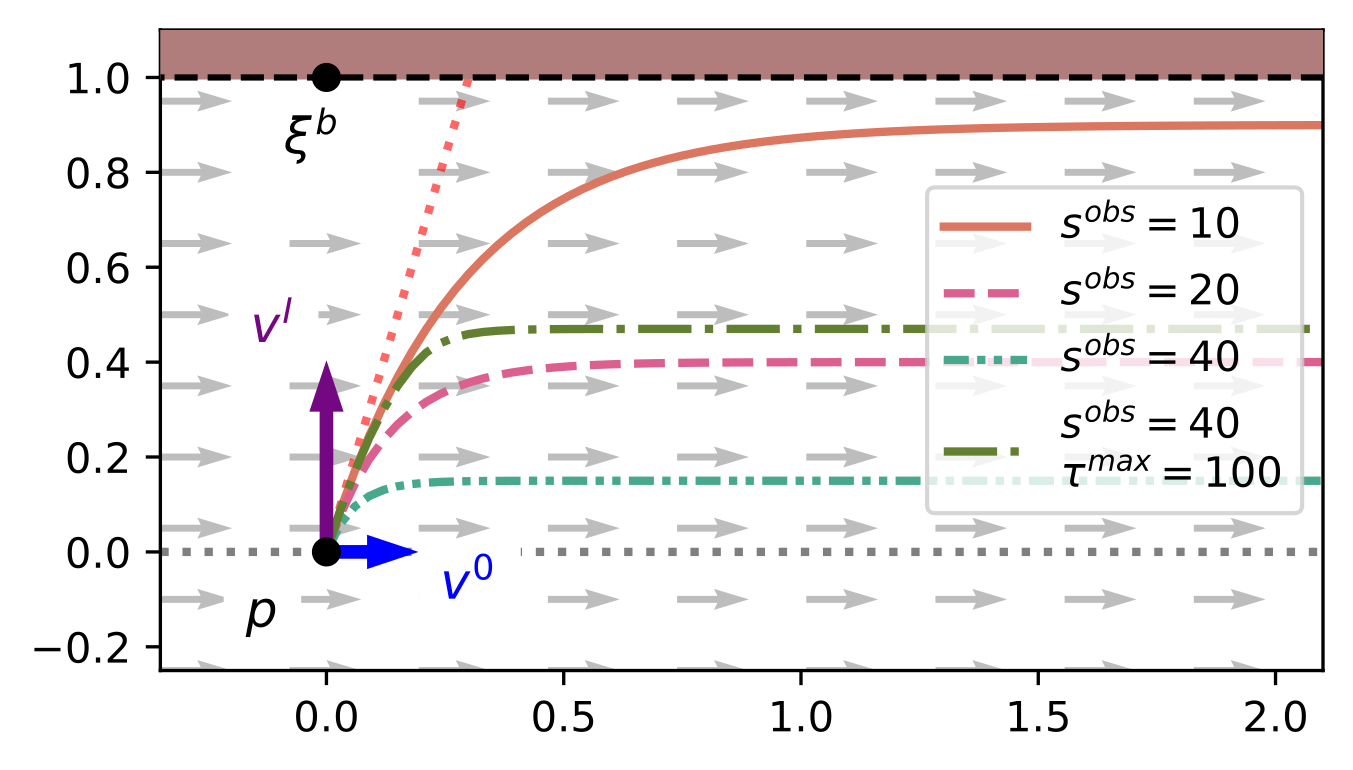
\includegraphics[width=0.99\columnwidth]{figures/parallel_avoidance_obstacle}}
  \caption{A disturbance occurs of a point-agent at position $\vect p^0$ with velocity after the impact of $\{ \dot{\vecs \xi} \}_0 = \vect v^0 + \vect v^I$. A high damping in the direction of the obstacle in the presence of a constant velocity field (gray) ensures collision avoidance. Whereas different damping values $s^{\mathrm{o}}$ and optionally a maximum repulsion force $\vecs \tau^{\mathrm{max}}$ lead to different trajectories.}
  \label{fig:disturbance_with_parallel_velocity}
% \end{subfigure}
\end{figure}
    
\begin{proof}
Since we assume a point-like agent, the mass matrix $\matd{M}(\vecs \xi)$ is constant, with diagonal values of $m$. The damping matrix in the proximity of a single obstacle is approximated as follows:
\begin{equation}
\Gamma(\vecs \xi) \approx 1
\; \underset{\eqref{eq:averaged_normal}, \, \eqref{eq:weight_function} } {\Rightarrow} \;
\begin{array}{l}
% \lim_{\Gamma(\vecs \xi) \rightarrow 1} \| \vect n(\vecs \xi) \| = 1, \\
% \lim_{\Gamma(\vecs \xi) \rightarrow 1}\; w(\vecs \xi) = 1
\| \vect n(\vecs \xi) \| = 1 \\
w(\vecs \xi) = 1
\end{array}
% \quad 
\underset{\eqref{eq:damping_summation}} {\Rightarrow} \quad
\matd D(\vecs \xi) = \matd{D}^o(\vecs \xi)
\end{equation}

Using the controller design from \eqref{eq:control_command} the velocity can be computed as:
\begin{equation}
\begin{split}
    \vecs{\dot \xi} & = \int \vecs{\ddot \xi} \, dt 
    = \int \matd{M}^{-1} \matd{D}  \left( \vecs{\dot \xi} - \vecs f(\vecs \xi) \right) \, dt \\
    % & \approx \int \matd{M}^{-1} \matd{D} \vect f(\vecs \xi) \, dt
\end{split}
\label{eq:velocity_evolution}
\end{equation}

Due to high velocity towards the obstacle after impact, relative to tangent velocity, i.e., $\| \vect v^I \| \gg \| \vect v^0 \|$, as well as the proximity to the obstacle from $\Gamma(\vecs \xi) \approx 1$, the agent is only able to move little before having to reject the disturbance. 
As a result, we can assume that the changes of the velocity field and the obstacle curvature are negligible, and hence we have $\vect f(\vecs \xi) = \text{const.}$ and $\vect n(\vecs \xi) = \text{const.}$
Using \eqref{eq:obstacle_damping_values} results in a constant damping matrix with damping values:
\begin{equation}
    \matd{S}^o_1 = s^o
    \; , \quad
    \matd{S}^o_2 = s^f
    \; , \quad
    \matd{S}^o_d = s^c \;\;\; d = 3 .. N
\end{equation}
From \eqref{eq:first_obstacle_basis}, we know that the first decomposition vector $\vect q_1^o(\vecs \xi)$ points along the normal $\vect n(\vecs \xi)$, and the second $\vect q_2^o(\vecs \xi)$ along the desired dynamics $\vect f(\vecs \xi)$.

% This allows for the analysis of the velocity from \eqref{eq:velocity_evolution} along decomposition direction $q_d^o$. In the tangent plane, the impact did not change the velocity, and hence:
% \begin{equation}
% \begin{split}
%     \dot{\vecs \xi}_d & = \int \matd{M}^{-1} \matd{D}  \left( \vecs f_d(\vecs \xi) - \vecs f_d(\vecs \xi) \right) \, dt  =  \vect v^0_d
%     %\qquad \text{with} \quad
% \end{split}
% \end{equation}
% with $d = 2 .. N$.

The velocity in the tangent plane does not lead to any impact. Hence, we can analyse the evolution of the velocity in the direction of the normal of the obstacle $\vecs{\dot \xi}_1$:
\begin{equation}
    \vecs{\dot \xi}_1 = \int \frac{s^{\mathrm{o}}}{m} \vecs{ \dot \xi}_1 \, dt = \frac{s^{\mathrm{o}}}{m} \left(\vecs{\xi}_1 - \vect p_1 \right)  + \vecs v^I_1 \label{eq:velocity_with_control}
\end{equation}
% where $m = \min \Bigl(\text{eig} \bigl(\mathcal{M} \bigr) \Bigr)$ is the smallest eigenvalue of the mass matrix. Note, that any velocity which does not point towards the surface, will not get as close to the obstacle.

This can be used to compute the position at which the velocity in the normal direction reaches zero:
\begin{equation}
    \| \vecs{\dot \xi} _1 \| = 0
    \quad \Rightarrow \quad
    \| \vecs{\xi}_1 -  \vect p_1 \| = \| \vecs v^I_1 \| {m} / {s^{\mathrm{o}}} 
\end{equation}

As long as the disturbance is limited by
\begin{equation}
    \| \vect v^I \| < s^{\mathrm{o}} \| \vecs \xi - \vecs \xi^b \| / m
\end{equation}
it will stop at the closest surface point $\vecs \xi^b \in \mathbb{R}^N$, and hence remain collision-free.
\end{proof}

Note that the analysis is done for proximity regions of the obstacle. In any case, the robot enters this proximity region before a collision can occur. Hence, the proposed analysis holds as a general collision avoidance insurance.

Similarly, while we specifically analyze disturbances along the normal of the obstacle, any velocity after the disturbance can be divided into a part towards the obstacle, and a part parallel to the surface. Where a velocity parallel to the obstacle does not pose any danger for collision.
Yet, there is no guarantee against drifting into obstacles in the presence of highly curved surfaces and velocity fields. This is further discussed during the experiments in Section~\ref{sec:position_noise}, where it is, however, observed that the increased damping towards the obstacle significantly reduces collision in such scenarios. 

% \subsection{Disturbance Repulsion with Force Limit}
All robotic systems have a maximum force that they can exert on the environment based on the motors and their geometry, $\tau_c^{\mathrm{max}} \in \mathbb{R}_{>0}$. Additionally, such force limits are often state-dependent. A limiting force decreases the impact velocity a controller can handle while ensuring collision avoidance (Fig.~\ref{fig:disturbance_with_parallel_velocity}). Nevertheless, a maximum control force can be interpreted as adapting damping, and hence, the passivity from Theorem~\ref{theorem:passivity} holds.


